\documentclass[problem]{mcs}

\begin{pcomments}
  \pcomment{FP_chains_scheduling}
  \pcomment{FP version of CP_chains_scheduling}
  \pcomment{from S02.final, F03.final}
\end{pcomments}

\pkeywords{
 chain
 antichain
 topological
 schedule
}

%%%%%%%%%%%%%%%%%%%%%%%%%%%%%%%%%%%%%%%%%%%%%%%%%%%%%%%%%%%%%%%%%%%%%
% Problem starts here
%%%%%%%%%%%%%%%%%%%%%%%%%%%%%%%%%%%%%%%%%%%%%%%%%%%%%%%%%%%%%%%%%%%%%

\begin{problem}
Sauron finds that conquering Middle Earth breaks down into a bunch of
tasks.  Each task can be completed by a horrible creature called a
\emph{Ringwraith} in exactly one week.  Sauron realizes the
prerequisite structure among the tasks defines a partial order.  He
has $n$ tasks in his partial order, with a maximum length chain of $t$
tasks.  

In order to complete all $n$ tasks in $t$ weeks, Sauron will need to
have crew of Ringwraiths working in parallel.  In answering the
following questions, do not make any assumptions about the values of
$n$ and $t$ besides $1 \leq t \leq n$.

\bparts

\ppart Write a simple formula involving $n$ and $t$ for the smallest
number of Ringwraiths that Sauron could possibly need.

\examspace[0.5in]

\begin{solution}
\[
\ceil{\frac{n}{t}}
\]

Each of the $n$ tasks must be completed in one of the $t$ weeks.
Thus, by the pigeonhole principle, at least $\ceil{n/t}$ must be
completed in some week, thus requiring at least this many Ringwraiths.

This bound can't be made larger, since a partial order with a single
length $t$ chain and the other $n-t$ tasks with no prerequisites
can be completed in time $t$ by doing $\ceil{n/t}$ each week.
\end{solution}

\ppart On the other hand, if Sauron is unlucky, he may need a crew of
Ringwraiths as large as $n - t + 1$ in order to conquer Middle Earth
in $t$ weeks.  Describe a partial order with $n$ tasks and maximum
length chain of $t$ that would require this many Ringwraiths.

\begin{solution}
There will be $n - t + 1$ Ringwraiths needed if there is an antichain
of $n - t + 1$ tasks that cannot be started until a chain of $t - 1$
tasks is completed, as in the following figure:
\begin{center}
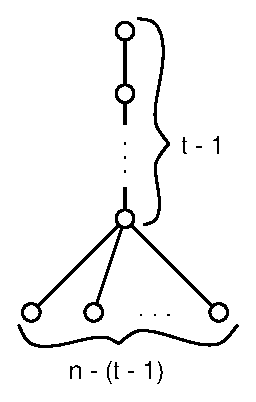
\includegraphics[height=2.5in]{pset5-hasse}
\end{center}
\end{solution}

\eparts

\end{problem}

%%%%%%%%%%%%%%%%%%%%%%%%%%%%%%%%%%%%%%%%%%%%%%%%%%%%%%%%%%%%%%%%%%%%%
% Problem ends here
%%%%%%%%%%%%%%%%%%%%%%%%%%%%%%%%%%%%%%%%%%%%%%%%%%%%%%%%%%%%%%%%%%%%%

\endinput
 
